\newpage
\usecaseristoratore{Assegnamento ingredienti ad un piatto}
\label{usecase:Assegnamento ingredienti ad un piatto}

\begin{figure}[h]
	\centering
	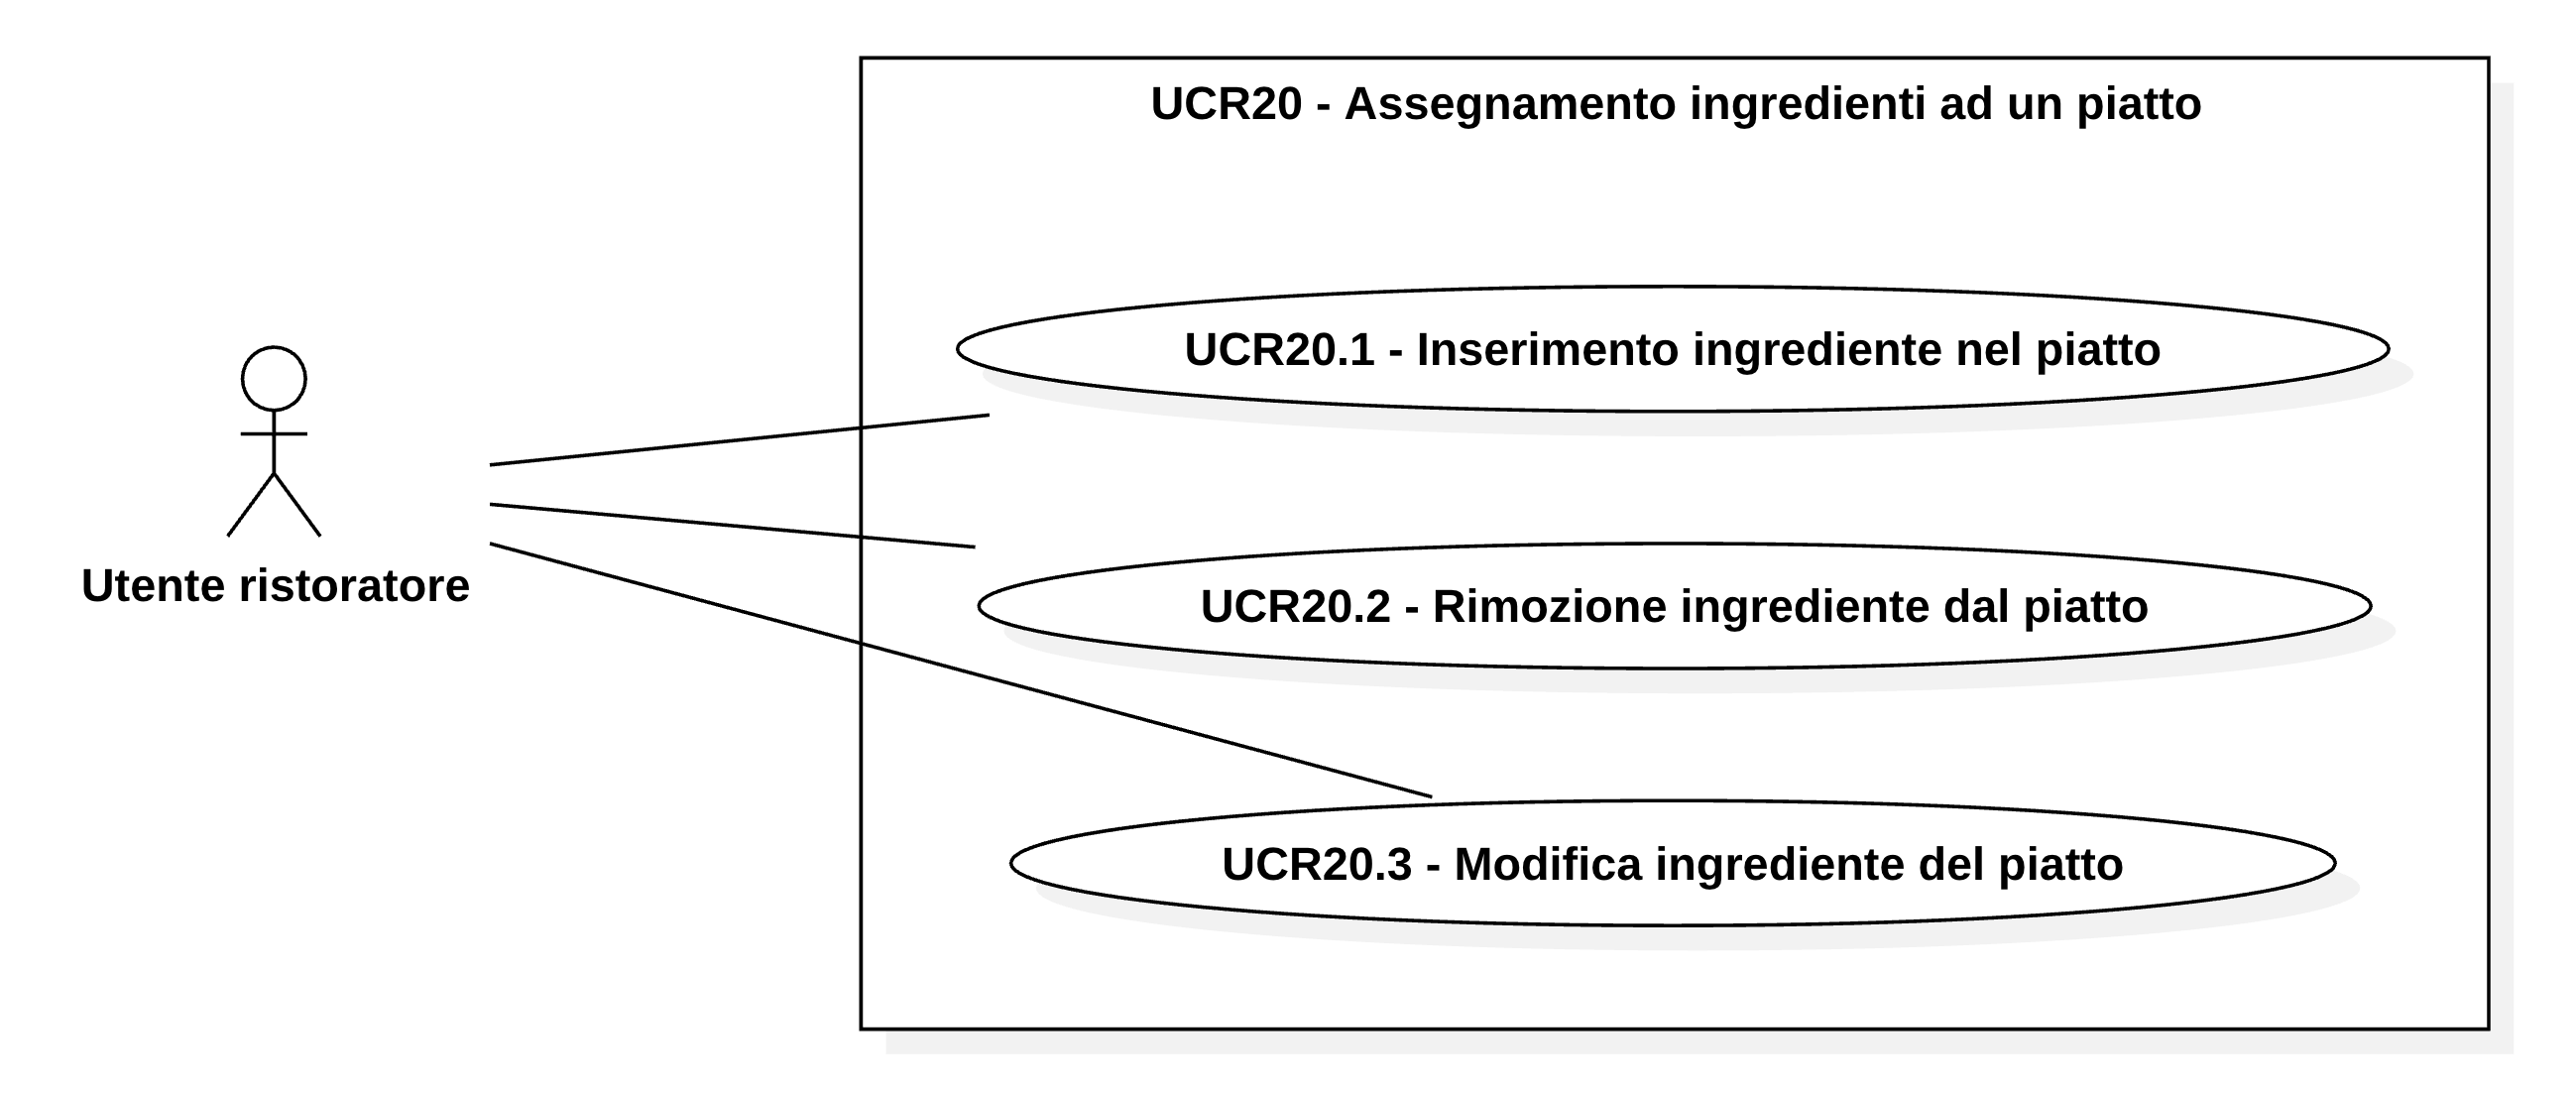
\includegraphics[width=0.9\textwidth]{./uml/UCR20.png} 
	\caption{Assegnamento ingredienti ad un piatto}
	\label{fig:UCR20}
  \end{figure}

\begin{itemize}
	\item \textbf{Attore principale:} Utente ristoratore.

	\item \textbf{Precondizione:} L'Utente ristoratore ha effettuato l'accesso al Sistema (vedi \autoref{usecase:Effettua accesso}).


	\item \textbf{Postcondizione:}
	      L'Utente ristoratore ha assegnato tutti gli ingredienti ad un piatto.

	\item \textbf{Scenario principale:}
	      \begin{enumerate}
			  \item L'Utente ristoratore può compiere le seguenti azioni per quanto riguarda la gestione degli ingredienti di un piatto:
				  \begin{itemize}
					  \item Inserimento di un ingrediente in un piatto (vedi \autoref{usecase:Inserimento ingrediente ad un piatto}).
					  \item Eliminazione di un ingrediente da un piatto (vedi \autoref{usecase:Eliminazione ingrediente da un piatto}).
					  \item Modifica di un ingrediente di un piatto (vedi \autoref{usecase:Modifica ingrediente di un piatto}).
				  \end{itemize}

		      \item Il Sistema registra gli ingredienti assegnati ad un piatto.
        \end{enumerate}
\end{itemize}

\subusecaseristoratore{Inserimento ingrediente nel piatto}
\label{usecase:Inserimento ingrediente ad un piatto}
\begin{itemize}

	\item \textbf{Attore principale:} Utente ristoratore.

	\item \textbf{Precondizione:} L'Utente ristoratore si trova nella sezione di gestione degli ingredienti di un piatto (vedi \autoref{usecase:Assegnamento ingredienti ad un piatto}).

	\item \textbf{Postcondizione:} L'Utente ristoratore ha inserito un
		ingrediente in un piatto.

	\item \textbf{Scenario principale:}
	\begin{enumerate}
		\item L'Utente ristoratore inserisce un ingrediente in un piatto;
		\item L'Utente deve specificare:
			\begin{itemize}
				\item L'ingrediente da assegnare;
				\item La quantità dell'ingrediente;
			\end{itemize}
		\item Il Sistema aggiorna la lista degli ingredienti assegnati ad un piatto.
	\end{enumerate}
\end{itemize}

\subusecaseristoratore{Eliminazione ingrediente dal piatto}
\label{usecase:Eliminazione ingrediente da un piatto}
\begin{itemize}

	\item \textbf{Attore principale:} Utente ristoratore.

	\item \textbf{Precondizione:} L'Utente ristoratore si trova nella sezione di gestione degli ingredienti di un piatto (vedi \autoref{usecase:Assegnamento ingredienti ad un piatto}).

	\item \textbf{Postcondizione:} L'Utente ristoratore ha eliminato un
		ingrediente dal piatto.

	\item \textbf{Scenario principale:}
	\begin{enumerate}
		\item L'Utente ristoratore elimina un ingrediente dal piatto;
		\item Il Sistema aggiorna la lista degli ingredienti assegnati ad un piatto.
	\end{enumerate}
\end{itemize}

\subusecaseristoratore{Modifica ingrediente del piatto}
\label{usecase:Modifica ingrediente di un piatto}
\begin{itemize}

	\item \textbf{Attore principale:} Utente ristoratore.

	\item \textbf{Precondizione:} L'Utente ristoratore si trova nella sezione di 
		gestione degli ingredienti di un piatto (vedi 
		\autoref{usecase:Assegnamento ingredienti ad un piatto}).

	\item \textbf{Postcondizione:} L'Utente ristoratore ha modificato un
		ingrediente di un piatto.

	\item \textbf{Scenario principale:}
	\begin{enumerate}
		\item L'Utente ristoratore modifica un ingrediente di un piatto;
		\item L'Utente può cambiare la quantità di un ingrediente assegnato ad un piatto;
		\item Il Sistema aggiorna la lista degli ingredienti assegnati ad un piatto.
	\end{enumerate}
\end{itemize}

